%
% Complete documentation on the extended LaTeX markup used for Insight
% documentation is available in ``Documenting Insight'', which is part
% of the standard documentation for Insight.  It may be found online
% at:
%
%     http://www.itk.org/

\documentclass{InsightArticle}

\usepackage[dvips]{graphicx}

%%%%%%%%%%%%%%%%%%%%%%%%%%%%%%%%%%%%%%%%%%%%%%%%%%%%%%%%%%%%%%%%%%
%
%  hyperref should be the last package to be loaded.
%
%%%%%%%%%%%%%%%%%%%%%%%%%%%%%%%%%%%%%%%%%%%%%%%%%%%%%%%%%%%%%%%%%%
\usepackage[dvips,
bookmarks,
bookmarksopen,
backref,
colorlinks,linkcolor={blue},citecolor={blue},urlcolor={blue},
]{hyperref}


%  This is a template for Papers to the Insight Journal.
%  It is comparable to a technical report format.

% The title should be descriptive enough for people to be able to find
% the relevant document.
\title{Conformal Flattening ITK Filter}

% Increment the release number whenever significant changes are made.
% The author and/or editor can define 'significant' however they like.
\release{0.00}

% At minimum, give your name and an email address.  You can include a
% snail-mail address if you like.
\author{Yi Gao$^{1}$ and et al $^{1}$ $^{2}$ $^{3}$}
\authoraddress{$^{1}$Georgia Institute of Technology, Atlanta, GA\\
               $^{2}$Kitware, Clifton Park, NY\\
               $^{3}$GE, Niskayuna, NY}

\begin{document}

\newif\ifpdf
\ifx\pdfoutput\undefined
  \pdffalse
\else
  \pdfoutput=1
  \pdftrue
\fi


\ifpdf
\else
   %
   % Commands for including Graphics when using latex
   %
   \DeclareGraphicsExtensions{.eps,.jpg,.gif,.tiff,.bmp,.png}
   \DeclareGraphicsRule{.jpg}{eps}{.jpg.bb}{`convert #1 eps:-}
   \DeclareGraphicsRule{.gif}{eps}{.gif.bb}{`convert #1 eps:-}
   \DeclareGraphicsRule{.tiff}{eps}{.tiff.bb}{`convert #1 eps:-}
   \DeclareGraphicsRule{.bmp}{eps}{.bmp.bb}{`convert #1 eps:-}
   \DeclareGraphicsRule{.png}{eps}{.png.bb}{`convert #1 eps:-}
\fi


\maketitle


\ifhtml
\chapter*{Front Matter\label{front}}
\fi


% The abstract should be a paragraph or two long, and describe the
% scope of the document.
\begin{abstract}
\noindent This document describes the Insight Toolkit (ITK)
Conformal Flattening filter.
\end{abstract}

\tableofcontents

Here we provide background on Conformal Flattening (angle
preserving, literature review, practical uses such as brain
flattening).

\section{Algorithm Details}

Here we provide details on the algorithm.


\section{User's Guide}

Here we provide details on the use of our filter.


\section{Examples}

Here we show examples of our filter in action.  We also provide
reviewers with all parameters and data so that they too can
reproduce our results.  This is crucial for a good review.


\section{Conclusions}

Here we summarize our work.


% The preceding sections will have been written in a gentler,
% introductory style.  You may also wish to include a reference
% section, documenting all the functions/exceptions/constants.
% Often, these will be placed in separate files and input like this:



%\appendix
%
%\section{This is an Appendix}
%
%To create an appendix in a Insight HOWTO document, use markup like
%this:
%
%\begin{verbatim}
%\appendix
%
%\section{This is an Appendix}
%
%To create an appendix in a Insight HOWTO document, ....
%
%
%\section{This is another}
%
%Just add another \section{}, but don't say \appendix again.
%\end{verbatim}


%%%%%%%%%%%%%%%%%%%%%%%%%%%%%%%%%%%%%%%%%%%%%%%%%%%%%%%%%%
%
%  Example on how to insert a figure
%
%%%%%%%%%%%%%%%%%%%%%%%%%%%%%%%%%%%%%%%%%%%%%%%%%%%%%%%%%%

%\begin{figure}
%\center
%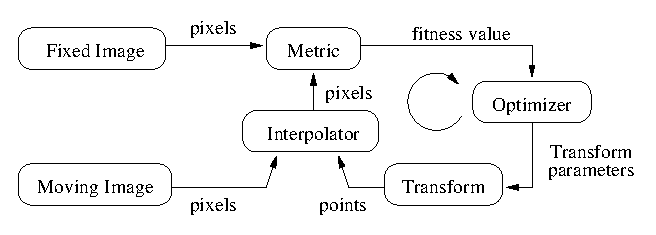
\includegraphics[width=0.8\textwidth]{RegistrationComponentsDiagram.eps}
%\itkcaption[Registration Framework Components]{The basic components of the
%registration framework are two input images, a transform, a metric, an
%interpolator and an optimizer.}
%\label{fig:RegistrationComponents}
%\end{figure}



%%%%%%%%%%%%%%%%%%%%%%%%%%%%%%%%%%%%%%%%%%%%%%%%%%%%%%%%%%
%
%  Example on how to insert an equation.
%  Never forget to put an equation in your paper.
%  They make them look professional and impress the reviewers.
%
%%%%%%%%%%%%%%%%%%%%%%%%%%%%%%%%%%%%%%%%%%%%%%%%%%%%%%%%%%


%To support shape-guidance, the generic level set equation
%(Eqn(~\ref{eqn:ShapeInfluenceTerm})) is extended to incorporate a shape guidance
%term:
%
%\begin{equation}
%\label{eqn:ShapeInfluenceTerm}
%\xi \left(\psi^{*}(\mathbf{x}) - \psi(\mathbf{x})\right)
%\end{equation}




%%%%%%%%%%%%%%%%%%%%%%%%%%%%%%%%%%%%%%%%%
%
%  Insert the bibliography using BibTeX
%
%%%%%%%%%%%%%%%%%%%%%%%%%%%%%%%%%%%%%%%%%

\bibliographystyle{plain}
\bibliography{InsightJournal}


\end{document}
